\documentclass{standalone}
\usepackage{tikz}
\usetikzlibrary{positioning}

\begin{document}

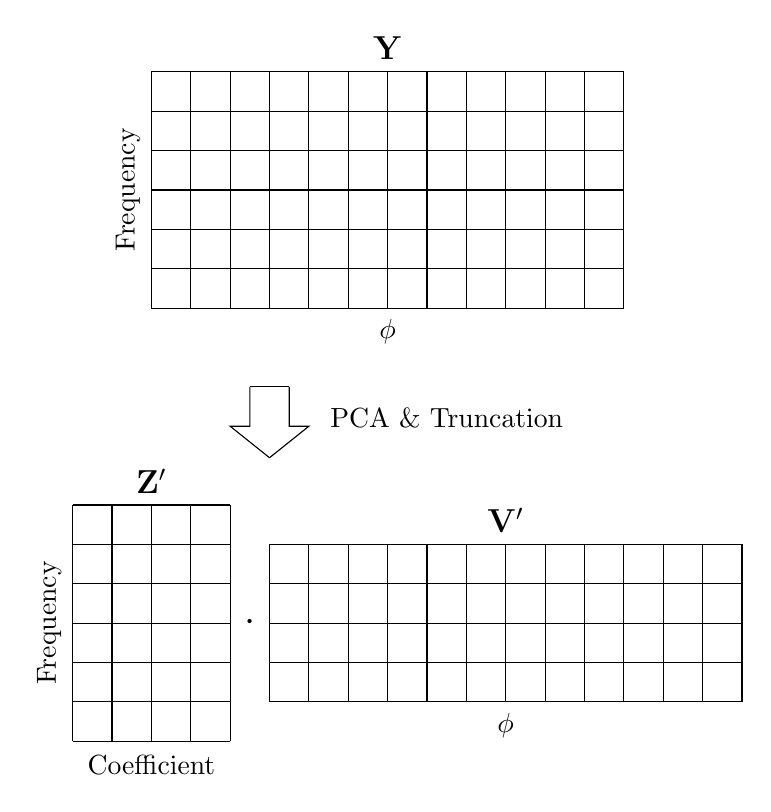
\begin{tikzpicture}[scale=.5]

\begin{scope}[shift={(2, 0)}]
    \draw[step=1, black] (0,0) grid (12,6);
    \node[yshift=-3mm] at (6, 0) {$\phi$};
    \node[xshift=-3mm, rotate=90] at (0, 3) {Frequency};
    \node[yshift=3mm] at (6, 6) {\large $\mathbf{Y}$};
\end{scope}

\begin{scope}[shift={(5, -2)}, rotate=-90]
    \draw[black] (0,+.5) -- ++(1, 0) -- ++(0, +.5) -- (1.8, 0);
    \draw[black] (0,-.5) -- ++(1, 0) -- ++(0, -.5) -- (1.8, 0);
    \draw[black] (0,-.5) -- (0,+.5);
\end{scope}
\begin{scope}[shift={(5, -2)}]
    \node at (4.5, -.8) {PCA \& Truncation};
\end{scope}

\begin{scope}[shift={(0, -11)}]
    \draw[step=1, black] (0,0) grid (4, 6);
    \node[yshift=-3mm] at (2, 0) {Coefficient};
    \node[xshift=-3mm, rotate=90] at (0, 3) {Frequency};

    \draw[step=1, black, shift={(5, 1)}] (0,0) grid (12,4);
    \node[yshift=-3mm] at (11, 1) {$\phi$};

    \node at (4.5, 3) {\Large $\cdot$};

    \node[yshift=3mm] at (2, 6) {\large $\mathbf{Z'}$};
    \node[yshift=3mm] at (11, 5) {\large $\mathbf{V'}$};
\end{scope}

\end{tikzpicture}

\end{document}
